%%%%%%%%%%%%%%%%%%%%%%%%%%%%%%%%%%%%%%%%%%%%%%%%%%%%%%%%%%%%%%%%%%%%%%%

\chapter{Experiment 2: Calculator Applications}

This chapter presents the implementation of a simple calculator using Arduino UNO, a 4×4 keypad, and an SSD1306 OLED display. The project demonstrates user input through a keypad, real-time arithmetic processing, and graphical output on an OLED display.

%%%%%%%%%%%%%%%%%%%%%%%%%%%%%%%%%%%%%%%%%%%%%%%%%%%%%%%%%%%%%%%%%%%%%%%

\section{Simple Calculator Using Arduino UNO}

%%%%%%%%%%%%%%%%%%%%%%%%%%%%%%%%%%%%%%%%%%%%%%%%%%%%%%%%%%%%%%%%%%%%%%%


\subsection{Problem Statement}

This project implements a simple calculator using Arduino UNO, a 4×4 keypad, and an SSD1306 OLED display. The calculator performs basic arithmetic operations such as addition, subtraction, multiplication, and division. The calculated result is displayed on the OLED screen in real time.

%%%%%%%%%%%%%%%%%%%%%%%%%%%%%%%%%%%%%%%%%%%%%%%%%%%%%%%%%%%%%%%%%%%%%%%

\subsection{Components Used \& Pin Connections}

\begin{table}[H]
\centering

\begin{minipage}[t]{0.48\textwidth}
\centering
\caption{Calculator Components}
\label{tab:calculator_components}

\begin{tabular}{|p{4cm}|c|}
\hline
\textbf{Component} & \textbf{Quantity} \\
\hline
Arduino UNO & 1 \\
4×4 Keypad & 1 \\
SSD1306 OLED Display & 1 \\
Jumper Wires & Required \\
Breadboard & 1 \\
\hline
\end{tabular}

\end{minipage}
\hfill
\begin{minipage}[t]{0.47\textwidth}
\centering
\caption{Keypad Pin Connections}
\label{tab:keypad_pins}

\begin{tabular}{|c|c|}
\hline
\textbf{Keypad Pin} & \textbf{Arduino Pin} \\
\hline
R1 & D1 \\
R2 & D2 \\
R3 & D3 \\
R4 & D4 \\
C1 & D5 \\
C2 & D6 \\
C3 & D7 \\
C4 & D8 \\
\hline
\end{tabular}

\end{minipage}

\end{table}

%%%%%%%%%%%%%%%%%%%%%%%%%%%%%%%%%%%%%%%%%%%%%%%%%%%%%%%%%%%%%%%%%%%%%%%

\subsection{OLED Display Connections}

\begin{table}[H]
\centering
\caption{SSD1306 OLED Display Connections}
\label{tab:oled_connections}

\begin{tabular}{|l|c|}
\hline
\textbf{OLED Pin} & \textbf{Arduino Pin} \\
\hline
VCC & 5V \\
GND & GND \\
SDA & A4 \\
SCL & A5 \\
\hline
\end{tabular}

\end{table}

%%%%%%%%%%%%%%%%%%%%%%%%%%%%%%%%%%%%%%%%%%%%%%%%%%%%%%%%%%%%%%%%%%%%%%%

\subsection{Keypad Operator Mapping}

\begin{table}[H]
\centering
\caption{Keypad Operator Mapping}
\label{tab:keypad_mapping}

\begin{tabular}{|c|c|}
\hline
\textbf{Symbol} & \textbf{Operation} \\
\hline
A & Addition (+) \\
B & Subtraction (-) \\
C & Multiplication (*) \\
D & Division (/) \\
\# & All Clear (AC) \\
\hline
\end{tabular}

\end{table}

%%%%%%%%%%%%%%%%%%%%%%%%%%%%%%%%%%%%%%%%%%%%%%%%%%%%%%%%%%%%%%%%%%%%%%%

\subsection{Software Used}

\begin{itemize}
    \item Arduino IDE
    \item SimulIDE
\end{itemize}

%%%%%%%%%%%%%%%%%%%%%%%%%%%%%%%%%%%%%%%%%%%%%%%%%%%%%%%%%%%%%%%%%%%%%%%

\subsection{Circuit Diagram}

\begin{figure}[H]
\centering

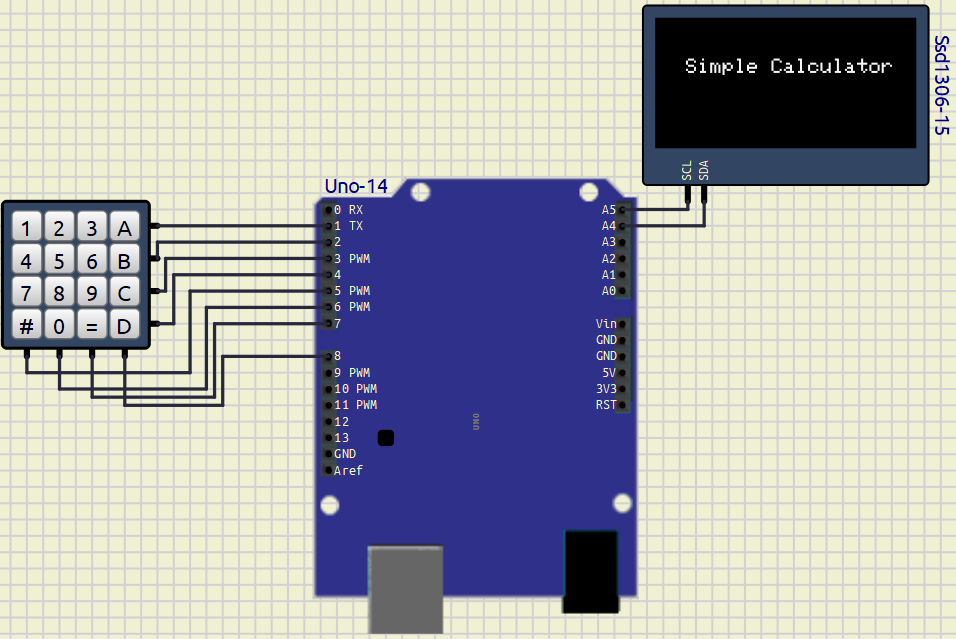
\includegraphics[width=0.55\textwidth]{Exp-2/Calculator/Start.png}

\caption{Simple Calculator Using Arduino UNO}
\label{fig:calculator}

\end{figure}

%%%%%%%%%%%%%%%%%%%%%%%%%%%%%%%%%%%%%%%%%%%%%%%%%%%%%%%%%%%%%%%%%%%%%%%

\subsection{Source Code}

The complete Arduino source code for this experiment is available in the project repository.

\href{https://github.com/YOUR_USERNAME/YOUR_REPOSITORY/blob/main/Exp-2/calculator/calculator.ino}
{\textbf{Click here to view the Arduino Source Code}}

%%%%%%%%%%%%%%%%%%%%%%%%%%%%%%%%%%%%%%%%%%%%%%%%%%%%%%%%%%%%%%%%%%%%%%%
%%%%%%%%%%%%%%%%%%%%%%%%%%%%%%%%%%%%%%%%%%%%%%%%%%%%%%%%%%%%%%%%%%%%%%%

\subsection{Working Principle}

\begin{enumerate}

\item The 4×4 keypad is used to enter numbers and arithmetic operators.

\item Arduino UNO continuously scans the keypad to detect key presses.

\item The entered numeric values are stored as operands.

\item The selected operator determines the arithmetic operation to be performed.

\item When the '=' key is pressed:

\begin{itemize}
    \item Arduino performs the requested calculation.
    \item The computed result is displayed on the SSD1306 OLED display.
\end{itemize}

\item Pressing the '\#' key clears all previous inputs and resets the calculator.

\item The calculator then becomes ready for the next calculation.

\end{enumerate}

%%%%%%%%%%%%%%%%%%%%%%%%%%%%%%%%%%%%%%%%%%%%%%%%%%%%%%%%%%%%%%%%%%%%%%%

\subsection{Output}

\begin{figure}[H]
\centering

\begin{minipage}{0.48\textwidth}
\centering
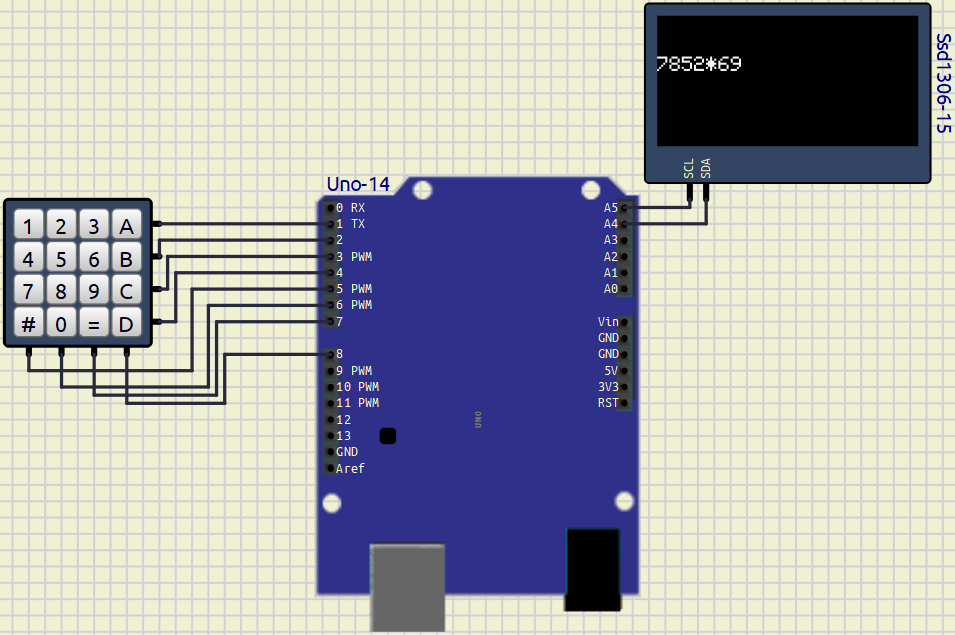
\includegraphics[width=\linewidth]{Exp-2/Calculator/Operation.png}
\\
\small (a) Arithmetic Operation
\end{minipage}
\hfill
\begin{minipage}{0.48\textwidth}
\centering
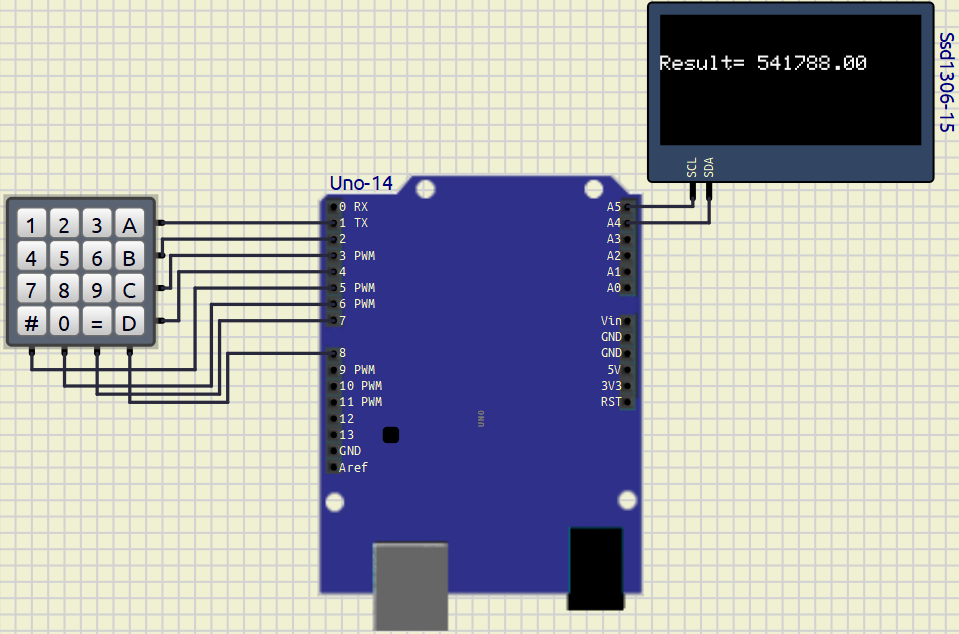
\includegraphics[width=\linewidth]{Exp-2/Calculator/Result.png}
\\
\small (b) Calculation Result
\end{minipage}

\caption{Calculator Operation and Output}
\label{fig:calculator_output}

\end{figure}

%%%%%%%%%%%%%%%%%%%%%%%%%%%%%%%%%%%%%%%%%%%%%%%%%%%%%%%%%%%%%%%%%%%%%%%

\subsection{Conclusion}

The Simple Calculator using Arduino UNO, a 4×4 Keypad, and an SSD1306 OLED Display was successfully implemented and tested.

The system successfully performs basic arithmetic operations, including addition, subtraction, multiplication, and division. User input is received through the keypad, and the calculated result is displayed on the OLED screen in real time.

During this experiment, the following concepts were learned:

\begin{itemize}

\item Matrix keypad interfacing

\item OLED display interfacing

\item User input processing

\item Arithmetic operation implementation

\item Embedded system programming

\end{itemize}

One challenge encountered during the implementation was mapping the keypad keys to their corresponding arithmetic operations. This issue was resolved by referring to the official Arduino documentation and open-source community resources.

%%%%%%%%%%%%%%%%%%%%%%%%%%%%%%%%%%%%%%%%%%%%%%%%%%%%%%%%%%%%%%%%%%%%%%%

\subsection{References}

\begin{enumerate}

\item Arduino Keypad Library Documentation

\url{https://www.arduino.cc/reference/en/libraries/keypad/}

\item Adafruit SSD1306 Library

\url{https://github.com/adafruit/Adafruit_SSD1306}

\item Arduino UNO Documentation

\url{https://docs.arduino.cc/hardware/uno-rev3/}

\item Adafruit GFX Graphics Library

\url{https://github.com/adafruit/Adafruit-GFX-Library}

\item 4×4 Keypad Arduino Code, Pinout \& Interfacing Guide

\url{https://robosans.com/learn/embedded/arduino/4x4-keypad-arduino-code-pinout-interfacing-lcd/}

\end{enumerate}

%%%%%%%%%%%%%%%%%%%%%%%%%%%%%%%%%%%%%%%%%%%%%%%%%%%%%%%%%%%%%%%%%%%%%%%
\clearpage

%%%%%%%%%%%%%%%%%%%%%%%%%%%%%%%%%%%%%%%%%%%%%%%%%%%%%%%%%%%%%%%%%%%%%%%

\clearpage
Experiment 2 (Go Further 1):
\section{BODMAS Method-Based Calculator}

%%%%%%%%%%%%%%%%%%%%%%%%%%%%%%%%%%%%%%%%%%%%%%%%%%%%%%%%%%%%%%%%%%%%%%%

\subsection{Problem Statement}

The objective of this project is to design a calculator using Arduino UNO, an SSD1306 OLED display, and a 5×4 matrix keypad that performs arithmetic calculations according to the BODMAS (Bracket, Order, Division, Multiplication, Addition, and Subtraction) rule.

The calculator evaluates mathematical expressions entered through the keypad and displays the calculated result on the OLED display. Additional features such as history, backspace, and expression clearing improve the usability of the system.

%%%%%%%%%%%%%%%%%%%%%%%%%%%%%%%%%%%%%%%%%%%%%%%%%%%%%%%%%%%%%%%%%%%%%%%

\subsection{Components Used \& Pin Connections}

\begin{table}[H]
\centering

%%%%%%%%%%%%%%%%%%%%%%%%%%%%%%%%%%%%%%%%%%%%%%%%%%%%%%%%%%%%%%%%%%%%%%%
% First Row
%%%%%%%%%%%%%%%%%%%%%%%%%%%%%%%%%%%%%%%%%%%%%%%%%%%%%%%%%%%%%%%%%%%%%%%

\begin{minipage}[t]{0.48\textwidth}
\centering
\caption{Components Used}
\label{tab:bodmas_components}

\begin{tabular}{|p{3.5cm}|c|}
\hline
\textbf{Component} & \textbf{Qty} \\
\hline
Arduino UNO & 1 \\
SSD1306 OLED Display & 1 \\
5×4 Matrix Keypad & 1 \\
Breadboard & 1 \\
Jumper Wires & Req. \\
\hline
\end{tabular}

\end{minipage}
\hfill
\begin{minipage}[t]{0.48\textwidth}
\centering
\caption{Keypad Connections}
\label{tab:bodmas_keypad}

\begin{tabular}{|c|c|}
\hline
\textbf{Pin} & \textbf{Arduino} \\
\hline
R1--R5 & D2--D6 \\
C1--C4 & D7--D10 \\
\hline
\end{tabular}

\end{minipage}

\vspace{0.6cm}


%%%%%%%%%%%%%%%%%%%%%%%%%%%%%%%%%%%%%%%%%%%%%%%%%%%%%%%%%%%%%%%%%%%%%%%
% Second Row
%%%%%%%%%%%%%%%%%%%%%%%%%%%%%%%%%%%%%%%%%%%%%%%%%%%%%%%%%%%%%%%%%%%%%%%

\begin{minipage}[t]{0.48\textwidth}
\centering
\caption{OLED Connections}
\label{tab:bodmas_oled}

\begin{tabular}{|c|c|}
\hline
\textbf{OLED Pin} & \textbf{Arduino} \\
\hline
SDA & A4 \\
SCL & A5 \\
\hline
\end{tabular}

\end{minipage}
\hfill
\begin{minipage}[t]{0.48\textwidth}
\centering
\caption{Keypad Functions}
\label{tab:bodmas_mapping}
\begin{tabular}{|c|l|}
\hline
\textbf{Key} & \textbf{Function} \\
\hline
A & Addition (+) \\
S & Subtraction (-) \\
M & Multiplication (*) \\
D & Division (/) \\
= & Calculate \\
\# & Clear \\
B & Backspace \\
H & History \\
\hline
\end{tabular}
\end{minipage}

\end{table}

%%%%%%%%%%%%%%%%%%%%%%%%%%%%%%%%%%%%%%%%%%%%%%%%%%%%%%%%%%%%%%%%%%%%%%%

\subsection{Software Used}

\begin{itemize}
    \item Arduino IDE
    \item SimulIDE
\end{itemize}

%%%%%%%%%%%%%%%%%%%%%%%%%%%%%%%%%%%%%%%%%%%%%%%%%%%%%%%%%%%%%%%%%%%%%%%

\subsection{Circuit Diagram}

\begin{figure}[H]
\centering

\begin{minipage}{0.48\textwidth}
\centering
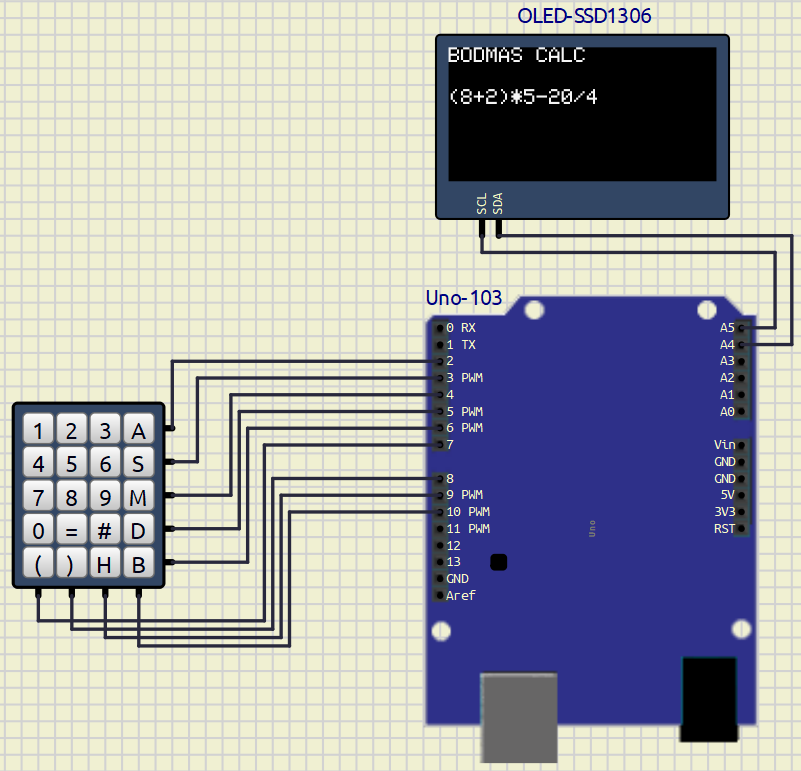
\includegraphics[width=\linewidth]{Exp-2/Calc_adv/circuit1.png}
\caption*{(a) Circuit Diagram - 1}
\end{minipage}
\hfill
\begin{minipage}{0.48\textwidth}
\centering
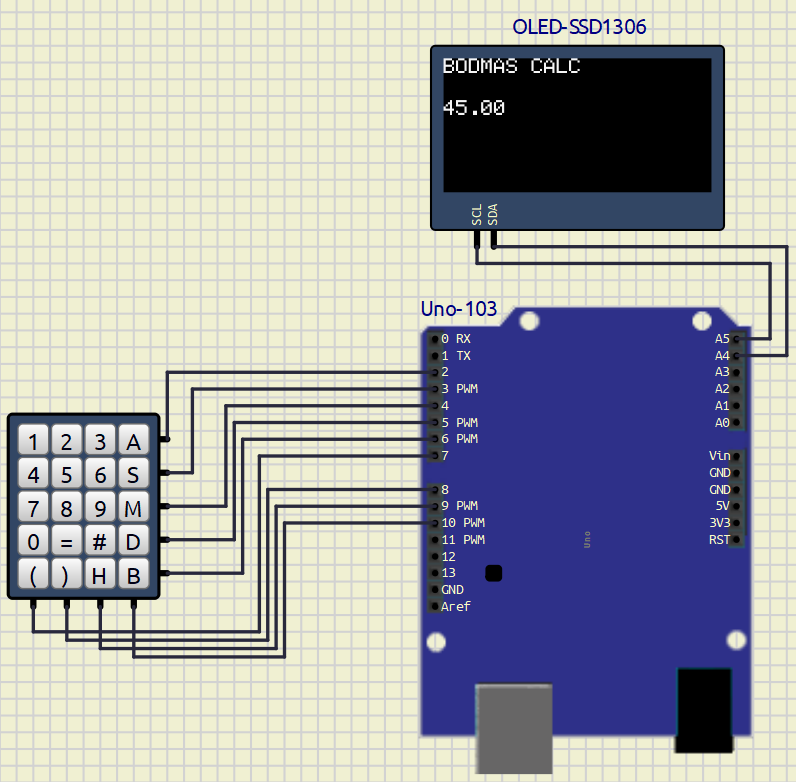
\includegraphics[width=\linewidth]{Exp-2/Calc_adv/circuit2.png}
\caption*{(b) Circuit Diagram - 2}
\end{minipage}

\caption{Circuit Diagram of the BODMAS Method Based Calculator}
\label{fig:bodmas_circuit}

\end{figure}

%%%%%%%%%%%%%%%%%%%%%%%%%%%%%%%%%%%%%%%%%%%%%%%%%%%%%%%%%%%%%%%%%%%%%%%

\subsection{Source Code}

The complete Arduino source code for this experiment is available in the project repository.

\href{https://github.com/YOUR_USERNAME/YOUR_REPOSITORY/blob/main/Exp-2/BODMAS_Calculator/BODMAS_Calculator.ino}
{\textbf{Click here to view the Arduino Source Code}}

%%%%%%%%%%%%%%%%%%%%%%%%%%%%%%%%%%%%%%%%%%%%%%%%%%%%%%%%%%%%%%%%%%%%%%%

%%%%%%%%%%%%%%%%%%%%%%%%%%%%%%%%%%%%%%%%%%%%%%%%%%%%%%%%%%%%%%%%%%%%%%%

\subsection{Working Principle}

\begin{enumerate}

\item The user enters a mathematical expression using the 5×4 matrix keypad.

\item Arduino UNO continuously scans the keypad and receives the entered input.

\item The entered mathematical expression is displayed on the SSD1306 OLED display in real time.

\item When the '=' key is pressed, Arduino evaluates the complete expression according to the BODMAS rule.

\item The calculated result is displayed on the OLED display.

\item Previous calculations are automatically stored in the history for future reference.

\item The '\#' key clears the current expression, while the 'B' key removes the last entered character (Backspace).

\item The 'H' key displays the calculation history stored in memory.

\end{enumerate}

%%%%%%%%%%%%%%%%%%%%%%%%%%%%%%%%%%%%%%%%%%%%%%%%%%%%%%%%%%%%%%%%%%%%%%%

\subsection{Output}

\textbf{Example Calculation}

\begin{table}[H]
\centering
\caption{Example BODMAS Calculation}
\label{tab:bodmas_output}

\begin{tabular}{|l|l|}
\hline
\textbf{Input Expression} & \texttt{(8+2)*5-20/4} \\
\hline
\textbf{Calculated Result} & \texttt{45} \\
\hline
\end{tabular}

\end{table}

The calculator successfully evaluated the mathematical expression according to the BODMAS rule and displayed the correct result on the OLED display.

%%%%%%%%%%%%%%%%%%%%%%%%%%%%%%%%%%%%%%%%%%%%%%%%%%%%%%%%%%%%%%%%%%%%%%%

\subsection{Conclusion}

The BODMAS Method-Based Calculator using Arduino UNO was successfully implemented and tested.

The calculator correctly evaluated mathematical expressions according to the BODMAS rule and displayed the calculated results on the SSD1306 OLED display. The addition of history, backspace, and expression-clearing features enhanced the calculator's usability and demonstrated efficient implementation of expression parsing in embedded systems.

During this experiment, the following concepts were learned:

\begin{itemize}

\item Matrix keypad interfacing

\item OLED display interfacing

\item Expression parsing

\item BODMAS rule implementation

\item Embedded system programming

\end{itemize}

%%%%%%%%%%%%%%%%%%%%%%%%%%%%%%%%%%%%%%%%%%%%%%%%%%%%%%%%%%%%%%%%%%%%%%%

\subsection{References}

\begin{enumerate}

\item Arduino Official Website

\url{https://www.arduino.cc/}

\item Arduino UNO Documentation

\url{https://docs.arduino.cc/hardware/uno-rev3/}

\item Adafruit SSD1306 Library

\url{https://github.com/adafruit/Adafruit_SSD1306}

\item Arduino Keypad Library

\url{https://playground.arduino.cc/Code/Keypad/}

\item CircuitBasics — Arduino Keypad Interfacing Guide

\url{https://www.circuitbasics.com/how-to-set-up-a-keypad-on-an-arduino/}

\end{enumerate}

%%%%%%%%%%%%%%%%%%%%%%%%%%%%%%%%%%%%%%%%%%%%%%%%%%%%%%%%%%%%%%%%%%%%%%%

\clearpage
Experiment 2 (Go Further 2):
\section{Digital Password Lock System}

%%%%%%%%%%%%%%%%%%%%%%%%%%%%%%%%%%%%%%%%%%%%%%%%%%%%%%%%%%%%%%%%%%%%%%%

\subsection{Project Name}

Digital Password Lock System using Arduino UNO, OLED Display, Keypad, LEDs, and Buzzer

%%%%%%%%%%%%%%%%%%%%%%%%%%%%%%%%%%%%%%%%%%%%%%%%%%%%%%%%%%%%%%%%%%%%%%%

\subsection{Problem Statement}

The objective of this project is to design and implement a Digital Password Lock System using Arduino UNO that provides secure password-based authentication.

The system allows a user to create a four-character password, authenticate access using the stored password, provide visual and audio feedback for successful and failed login attempts, and support secure password reset functionality. A three-attempt security mechanism is also implemented to improve system security.

%%%%%%%%%%%%%%%%%%%%%%%%%%%%%%%%%%%%%%%%%%%%%%%%%%%%%%%%%%%%%%%%%%%%%%%

\subsection{Components Used \& Pin Connections}

\begin{table}[H]
\centering

\begin{minipage}[t]{0.48\textwidth}
\centering
\caption{Password Lock Components}
\label{tab:password_components}

\begin{tabular}{|p{4cm}|c|}
\hline
\textbf{Component} & \textbf{Quantity} \\
\hline
Arduino UNO & 1 \\
SSD1306 OLED Display (I2C) & 1 \\
4×5 Matrix Keypad & 1 \\
Red LED & 1 \\
Green LED & 1 \\
Buzzer & 1 \\
Breadboard & 1 \\
Connecting Wires & As Required \\
USB Cable & 1 \\
\hline
\end{tabular}

\end{minipage}
\hfill
\begin{minipage}[t]{0.47\textwidth}
\centering
\caption{LED \& Buzzer Connections}
\label{tab:password_led}

\begin{tabular}{|l|c|}
\hline
\textbf{Component} & \textbf{Arduino Pin} \\
\hline
Buzzer & D11 \\
Green LED & D12 \\
Red LED & D13 \\
\hline
\end{tabular}

\end{minipage}

\end{table}

%%%%%%%%%%%%%%%%%%%%%%%%%%%%%%%%%%%%%%%%%%%%%%%%%%%%%%%%%%%%%%%%%%%%%%%

\subsection{OLED Display Connections}

\begin{table}[H]
\centering
\caption{OLED Display Connections}
\label{tab:password_oled}

\begin{tabular}{|l|c|}
\hline
\textbf{OLED Pin} & \textbf{Arduino Pin} \\
\hline
VCC & 5V \\
GND & GND \\
SDA & A4 \\
SCL & A5 \\
\hline
\end{tabular}

\end{table}

%%%%%%%%%%%%%%%%%%%%%%%%%%%%%%%%%%%%%%%%%%%%%%%%%%%%%%%%%%%%%%%%%%%%%%%

\subsection{Keypad Connections}

\begin{table}[H]
\centering
\caption{4×5 Matrix Keypad Connections}
\label{tab:password_keypad}

\begin{tabular}{|c|c|}
\hline
\textbf{Keypad Pin} & \textbf{Arduino Pin} \\
\hline
R1 & D2 \\
R2 & D3 \\
R3 & D4 \\
R4 & D5 \\
R5 & D6 \\
C1 & D7 \\
C2 & D8 \\
C3 & D9 \\
C4 & D10 \\
\hline
\end{tabular}

\end{table}

%%%%%%%%%%%%%%%%%%%%%%%%%%%%%%%%%%%%%%%%%%%%%%%%%%%%%%%%%%%%%%%%%%%%%%%

\subsection{Software Used}

\begin{itemize}
    \item Arduino IDE
    \item SimulIDE
\end{itemize}

%%%%%%%%%%%%%%%%%%%%%%%%%%%%%%%%%%%%%%%%%%%%%%%%%%%%%%%%%%%%%%%%%%%%%%%

\subsection{Circuit Diagram}

\begin{figure}[H]
\centering

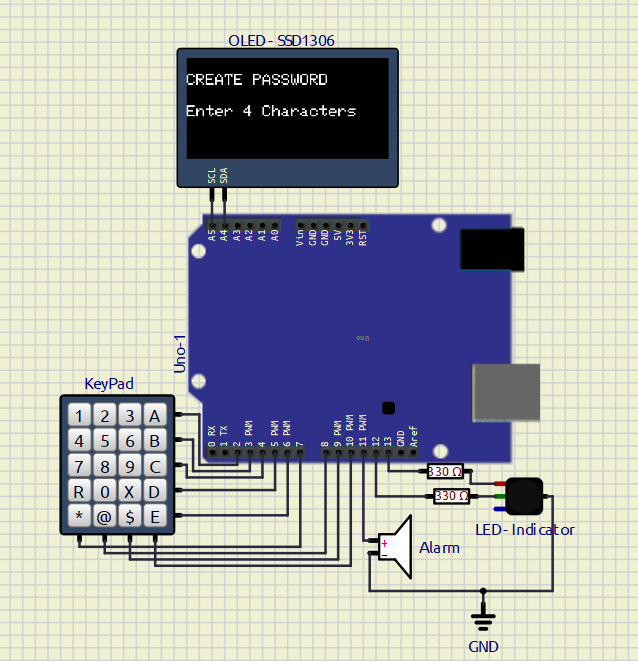
\includegraphics[width=0.60\textwidth]{Exp-2/digi_lock/circuit.png}

\caption{Digital Password Lock System Circuit Diagram}
\label{fig:password_lock}

\end{figure}

%%%%%%%%%%%%%%%%%%%%%%%%%%%%%%%%%%%%%%%%%%%%%%%%%%%%%%%%%%%%%%%%%%%%%%%

\subsection{Source Code}

The complete Arduino source code for this experiment is available in the project repository.

\href{https://github.com/YOUR_USERNAME/YOUR_REPOSITORY/blob/main/Exp-2/Password_Lock_System/password_lock_system.ino}
{\textbf{Click here to view the Arduino Source Code}}

%%%%%%%%%%%%%%%%%%%%%%%%%%%%%%%%%%%%%%%%%%%%%%%%%%%%%%%%%%%%%%%%%%%%%%%
%%%%%%%%%%%%%%%%%%%%%%%%%%%%%%%%%%%%%%%%%%%%%%%%%%%%%%%%%%%%%%%%%%%%%%%

\subsection{Working Principle}

\begin{enumerate}

\item When the system is powered ON, the user is prompted to create a four-character administrator password.

\item The entered password is securely stored in the Arduino memory and is used for future authentication.

\item During login, the user enters the password using the 4×5 matrix keypad.

\item Each key press is represented by an asterisk (*) on the OLED display to protect the password from being viewed.

\item If the entered password matches the stored password:

\begin{itemize}
    \item Access is granted.
    \item The green LED turns ON.
    \item A success beep is generated using the buzzer.
\end{itemize}

\item If an incorrect password is entered:

\begin{itemize}
    \item Access is denied.
    \item The red LED turns ON.
    \item An error beep is generated.
    \item The remaining login attempts are displayed on the OLED screen.
\end{itemize}

\item After three consecutive incorrect password attempts:

\begin{itemize}
    \item The system enters Alarm Mode.
    \item The red LED blinks continuously.
    \item The buzzer sounds continuously.
    \item The system remains locked until reset.
\end{itemize}

\item The password can be reset securely by pressing the \texttt{R} key and entering the existing password before creating a new password.

\end{enumerate}

%%%%%%%%%%%%%%%%%%%%%%%%%%%%%%%%%%%%%%%%%%%%%%%%%%%%%%%%%%%%%%%%%%%%%%%

\subsection{System Output}

\begin{table}[H]
\centering
\caption{Digital Password Lock System Output}
\label{tab:password_output}

\begin{tabular}{|p{5cm}|p{7.5cm}|}
\hline
\textbf{System State} & \textbf{OLED Display} \\
\hline
System Startup & SET ADMIN PASS \\ Enter 4 Characters \\
\hline
Password Saved & PASSWORD SAVED \\ System Ready \\
\hline
User Login & ENTER PASSWORD \\ Unlock The System \\
\hline
Correct Password & ACCESS GRANTED \\
\hline
Wrong Password & ACCESS DENIED \\ LEFT: 2 \\
\hline
Alarm Mode & SYSTEM LOCKED \\ PRESS R RESET \\
\hline
Password Reset & RESET PASSWORD \\ Enter Old Pass \\
\hline
Reset Successful & CORRECT PASSWORD \\ Set New Pass \\
\hline
\end{tabular}

\end{table}

%%%%%%%%%%%%%%%%%%%%%%%%%%%%%%%%%%%%%%%%%%%%%%%%%%%%%%%%%%%%%%%%%%%%%%%

\subsection{Problems Faced}

\begin{itemize}

\item OLED display address mismatch (0x3C / 0x3D).

\item Incorrect SDA and SCL wiring.

\item Keypad row and column mapping errors.

\item Undefined LED pin names during coding.

\item OLED text overflow due to long messages.

\item Alarm mode creating an infinite loop during debugging.

\item Password reset functionality required additional verification logic.

\item Synchronizing keypad input with OLED display updates.

\end{itemize}

%%%%%%%%%%%%%%%%%%%%%%%%%%%%%%%%%%%%%%%%%%%%%%%%%%%%%%%%%%%%%%%%%%%%%%%

\subsection{Conclusion}

The Digital Password Lock System using Arduino UNO was successfully implemented and tested.

The system provides secure password-based authentication using a matrix keypad and OLED display. Visual feedback through LEDs, audio indication using a buzzer, and a three-attempt security mechanism improve both usability and system security. The password reset feature further enhances flexibility while maintaining secure access control.
\clearpage
During this experiment, the following concepts were learned:
\begin{itemize}

\item Matrix keypad interfacing

\item OLED display interfacing

\item Password authentication

\item Embedded security systems

\item User access control

\item Alarm system implementation

\end{itemize}

%%%%%%%%%%%%%%%%%%%%%%%%%%%%%%%%%%%%%%%%%%%%%%%%%%%%%%%%%%%%%%%%%%%%%%%

\subsection{References}

\begin{enumerate}

\item SSD1306 OLED Display Datasheet

\url{https://cdn-shop.adafruit.com/datasheets/SSD1306.pdf}

\item Matrix Keypad Working Principle

\url{https://www.electronicsforu.com/technology-trends/learn-electronics/keypad-interfacing-arduino}

\item I2C Communication Protocol Overview

\url{https://lastminuteengineers.com/i2c-lcd-arduino-tutorial/}

\item Password-Based Access Control Systems

\url{https://circuitdigest.com/microcontroller-projects/password-based-door-lock-system-using-arduino}

\item Matrix Keypad Scanning Technique

\url{https://www.geeksforgeeks.org/keypad-interfacing-with-arduino/}

\item Buzzer and Alarm Circuit Concepts

\url{https://components101.com/modules/buzzer-module}

\end{enumerate}

%%%%%%%%%%%%%%%%%%%%%%%%%%%%%%%%%%%%%%%%%%%%%%%%%%%%%%%%%%%%%%%%%%%%%%%

\clearpage